\documentclass[12pt]{article}
\usepackage[utf8]{inputenc}
\usepackage{graphicx}
\usepackage{hyperref}
\usepackage{float}

\title{Simulación de eventos discretos}

\author{
  Autores :\\
  Amanda Noris Hernández \\
  Juan Miguel Pérez Martínez \\
  Marcos Antonio Pérez Lorenzo\\
}
\begin{document}
\maketitle


\section{Introducción}

\subsection{Descripción del problema}
Este proyecto se enfoca en la simulación de un sistema que cuenta con (n) servidores en paralelo, donde los clientes llegan de manera aleatoria siguiendo una distribución (M) para el tiempo entre llegadas. Los servidores se encargan de atender a los clientes, y el sistema maneja la asignación de clientes a servidores de manera que se minimice el tiempo de espera y abandonada del sistema. La simulación aborda cómo la distribución de servicio en cada servidor, representada por (Gi), afecta el rendimiento del sistema.

\subsection{Objetivos y metas}
\begin{enumerate}
\item Analizar el rendimiento del sistema: Evaluar cómo la asignación de clientes entre servidores afecta el tiempo de espera y abandonada del sistema.
\item Optimizar la distribución de servicio: Determinar la distribución óptima de servicio en cada servidor para minimizar el tiempo promedio de espera y abandonada del sistema.
\item Modelar la llegada de clientes: Utilizar la distribución (M) para modelar la llegada de clientes al sistema, y cómo esto influye en el comportamiento del sistema.
\item Simular el sistema en condiciones reales: Utilizar la simulación para modelar el comportamiento del sistema en condiciones reales, permitiendo la adaptación y optimización del modelo basado en los resultados.
\end{enumerate}

\subsection{Variables de interés}
Las variables de interés incluyen:
\begin{enumerate}

\item cycleCount: El número de ciclos completados en la simulación. Un ciclo puede representar un intervalo de tiempo o una iteración específica en el proceso de simulación.
\item maxClientsInQueue: El número máximo de clientes que se han encolado en la simulación. Este valor indica el pico de la demanda que el sistema ha experimentado.
\item maxClientWaitTime: El tiempo de espera máximo que un cliente ha tenido que esperar para ser atendido. Este valor es crítico para evaluar la eficiencia del sistema, ya que tiempos de espera largos pueden afectar negativamente la experiencia del cliente.
\item meanClientWaitTime: El tiempo promedio de espera de los clientes. Proporciona una medida de la eficiencia del sistema en términos de tiempo de servicio medio.
\item totalClientsServed: El número total de clientes que han sido atendidos durante la simulación. Este valor indica la capacidad de procesamiento del sistema a lo largo del tiempo.
\item totalWaitTime: El tiempo total de espera acumulado por todos los clientes. Este valor puede ser útil para calcular la eficiencia del sistema en términos de tiempo total de espera.
\item totalUsageTime: El tiempo total de uso del servidor acumulado. Este valor puede ayudar a entender cómo se distribuye el tiempo de trabajo entre los servidores.
\item averageServiceTimePerClient: El tiempo promedio de servicio por cliente. Este valor es crucial para evaluar la eficiencia del sistema en términos de tiempo de servicio.
\item max-client, min-client, max-server, min-server: Estos parámetros representan los valores máximos y mínimos para la cantidad de clientes y servidores en la simulación. Estos valores definen los límites del sistema y pueden influir en cómo se comporta bajo diferentes condiciones de carga.
\item initial number of simulated clients: El número inicial de clientes simulados al inicio de la simulación. Este valor establece el punto de partida para la demanda en el sistema.
\item number of simulated servers: El número de servidores simulados en la simulación. Este valor define la capacidad de procesamiento del sistema.
\item distribution for all service's time, distribution for i-nth service's time, distribution for client arrival time: Estos parámetros describen las distribuciones utilizadas para generar los tiempos de servicio y llegada de los clientes. Estas distribuciones pueden ser importantes para modelar variabilidad en el sistema.
\item duration: La duración de la simulación. Este valor indica el tiempo total durante el cual se ejecutó la simulación.

\end{enumerate}

\section{Detalles de implementación}

El proyecto se divide en varios módulos que se encargan de correr las simulaciones y de realizar análisis a partir de los datos obtenidos de las mismas.

El módulo distributions proporciona funciones para generar números aleatorios que siguen diferentes distribuciones estadísticas, lo cual es fundamental para modelar variabilidad en procesos simulados. Este módulo define cuatro funciones principales que representan cuatro tipos de distribuciones: uniforme, normal, de Poisson y exponencial. Cada una de estas funciones toma como argumentos los límites o parámetros específicos de la distribución, como los valores mínimo y máximo para la distribución uniforme, o la media y la desviación estándar para la distribución normal. Estas funciones son útiles para simular eventos con diferentes patrones de ocurrencia, como tiempos de llegada de clientes o tiempos de servicio en un sistema de simulación. Al utilizar estas distribuciones, el módulo permite modelar sistemas reales de manera más precisa, capturando la variabilidad inherente en los tiempos de eventos. Siempre que se desee, se pueden agregar más distribuciones para ampliar el rango de experimentos.

El módulo simulation proporciona una implementación básica de una simulación que modela un sistema de clientes y servidores. Este módulo define clases para representar a los clientes y servidores, así como para la simulación en sí misma. La clase Simulation gestiona la lógica principal de la simulación, incluyendo el manejo de la cola de clientes, la asignación de clientes a servidores, y el seguimiento de métricas clave como el tiempo total de servicio y el número de clientes atendidos. La simulación se ejecuta durante un tiempo especificado, actualizando el estado del sistema en cada ciclo. Este módulo es fundamental para modelar y analizar sistemas de procesamiento de solicitudes, permitiendo a los usuarios entender cómo diferentes configuraciones y parámetros afectan el rendimiento del sistema.

El módulo simulation-servers es responsable de configurar y ejecutar una simulación basada en clientes y servidores, utilizando argumentos de línea de comando para personalizar la simulación. Este módulo utiliza la biblioteca argparse para analizar los argumentos de línea de comando, que incluyen parámetros como el número máximo y mínimo de clientes y servidores, la cantidad inicial de clientes, la duración de la simulación, y las distribuciones utilizadas para los tiempos de llegada de los clientes y los tiempos de servicio. Con estos parámetros, el módulo configura las distribuciones de tiempo para los servicios y los tiempos de llegada de los clientes, crea una instancia de la simulación utilizando la clase CursesSimulation, inicia los clientes, y ejecuta la simulación durante el tiempo especificado. Al final de la simulación, imprime y guarda los resultados, que incluyen métricas como el número de ciclos completados, el número máximo de clientes en cola, el tiempo máximo de espera de un cliente, el tiempo promedio de espera de los clientes, el número total de clientes atendidos, el tiempo total de espera, el tiempo total de uso de los servidores, y el tiempo promedio de servicio por cliente. Estos resultados proporcionan una evaluación del rendimiento del sistema simulado bajo las condiciones especificadas.

El módulo curses-simulation extiende la clase StatSimulation para agregar capacidades de visualización en tiempo real de la simulación utilizando la biblioteca curses de Python. Este módulo es específicamente diseñado para proporcionar una interfaz gráfica basada en texto para visualizar el estado de la simulación en la terminal. Al hacerlo, permite una mejor comprensión y seguimiento del comportamiento del sistema simulado durante su ejecución. Las funciones clave en CursesSimulation incluyen inicializar la pantalla de curses (curses.initscr()), manejar interrupciones de teclado para terminar la simulación de manera limpia, y actualizar la pantalla para reflejar el estado actual de la simulación, como la cola de clientes, el estado de los servidores (ocupados, inactivos, terminando un servicio), y el número de clientes en cola. Estas actualizaciones visuales se realizan en tiempo real, permitiendo a los usuarios monitorear la simulación mientras se ejecuta.

El módulo data-recopilation es responsable de ejecutar simulaciones aleatorias de un sistema utilizando diferentes parámetros generados aleatoriamente para evaluar su comportamiento bajo una variedad de condiciones. Este módulo utiliza la función random-simulation para generar valores aleatorios para los parámetros de la simulación, como el número máximo y mínimo de clientes y servidores, la distribución de tiempos de llegada de clientes, tiempos de servicio, y la duración de la simulación. Estos parámetros son luego pasados a la función run-simulation del módulo serversRunner para ejecutar la simulación con estos valores aleatorios. Finalmente, el módulo ejecuta la función random-simulation 100 (este valor puede ser evidentemente modificado) veces en un bucle, lo que permite recopilar una gran cantidad de datos sobre el comportamiento del sistema bajo diferentes condiciones, facilitando el análisis y la mejora de su rendimiento.

El módulo simulation-stats proporciona una implementación de una clase StatSimulation que extiende una clase base Simulation. Esta clase se centra en recopilar y calcular estadísticas clave de una simulación, como el número de ciclos completados, el número máximo de clientes en cola, el tiempo de espera máximo de un cliente, el tiempo total de espera y de servicio, y el tiempo promedio de servicio por cliente. Estas estadísticas son fundamentales para evaluar el rendimiento del sistema simulado bajo diferentes condiciones. Además, el módulo incluye una función save que permite guardar los resultados de la simulación en un archivo CSV, facilitando el análisis y la comparación de los resultados de múltiples ejecuciones de la simulación. Este módulo es crucial para cualquier proyecto de simulación que requiera un análisis detallado del comportamiento del sistema bajo diferentes configuraciones y condiciones de carga.

El módulo stats-analysis se centra en el análisis estadístico de los datos recopilados de una simulación, utilizando bibliotecas de Python como pandas, numpy, matplotlib, seaborn y scipy para cargar, visualizar y analizar los datos. El análisis comienza cargando los datos desde un archivo CSV, que contiene los resultados de múltiples ejecuciones de la simulación. Luego, se presentan resúmenes y estadísticas descriptivas de los datos, incluyendo el número de filas, las columnas, y un resumen estadístico para cada columna. Se calculan y muestran estimaciones básicas estadísticas para varias métricas clave, como el tiempo máximo de espera del cliente, el tiempo promedio de servicio por cliente, el número máximo de clientes en cola, y el número total de clientes atendidos, utilizando métodos como la media, la desviación estándar y la varianza. Además, se realizan análisis de correlación entre las variables numéricas y comparaciones entre las diferentes distribuciones utilizadas. Se tiene en cuenta de otras variables su distribución aunque no se haya definido explícitamente o no se tenga conocimiento de la misma anteriormente. Este módulo es crucial para entender y analizar el rendimiento del sistema simulado, identificando tendencias, patrones y relaciones entre las diferentes métricas recopiladas.


\section{Resultados y experimentos}
\subsection{Hallazgos de la simulación e interpretación de los resultados}
 
 Se realizaron aproximadamente 100 experimentos de simulación con valores aleatorios de parámetros para llevar a cabo un análisis estadístico posterior. Los datos recopilados fueron almacenados en el archivo results.csv .

\begin{figure}[H]
\centering
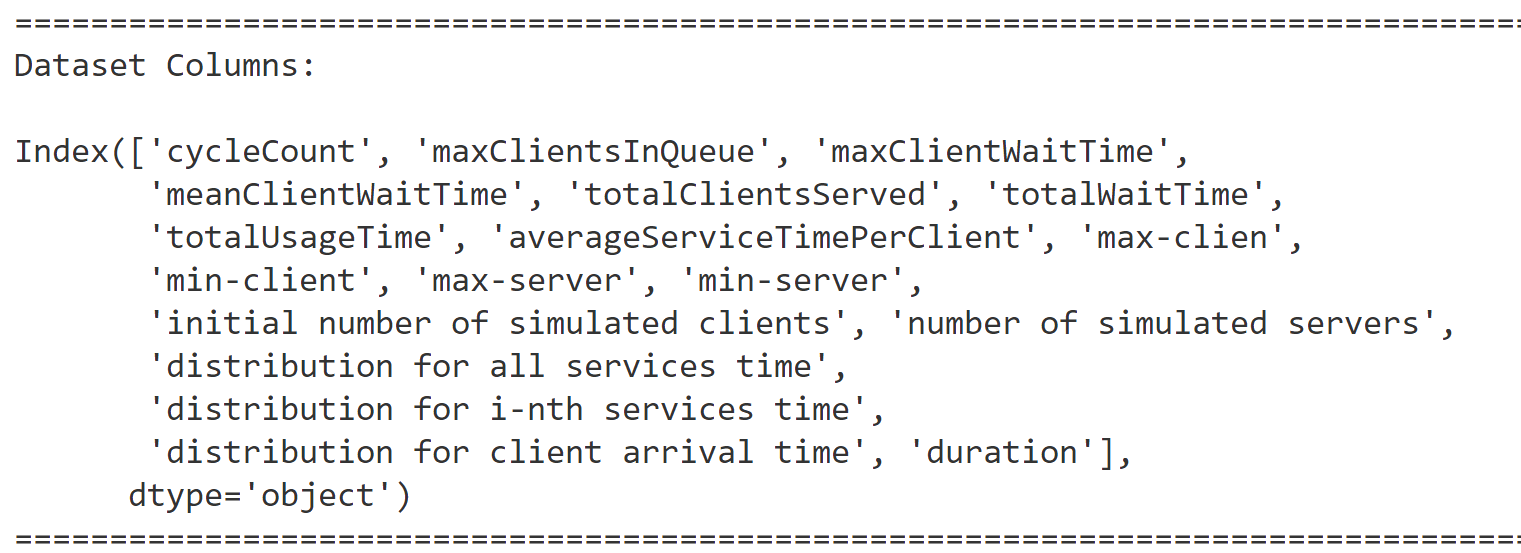
\includegraphics[width=1.2\textwidth]{columnas.png}
\caption{Columnas de la base de datos}
\end{figure}

\begin{figure}[H]
\centering
\includegraphics[width=1.2\textwidth]{descripción.png}
\caption{Descripción de la base de datos}
\end{figure}

 También se extrajo información más específica de algunas de las variables analizadas.

\begin{figure}[H]
\centering
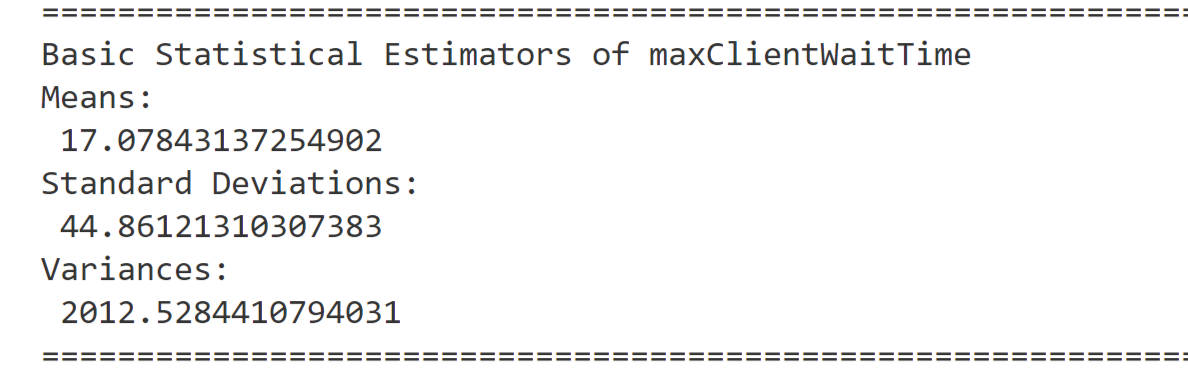
\includegraphics[width=1.2\textwidth]{tiempo de espera estimadores.png}
\caption{Estimadores de la variable tiempo de espera máximo}
\end{figure}

\begin{figure}[H]
\centering
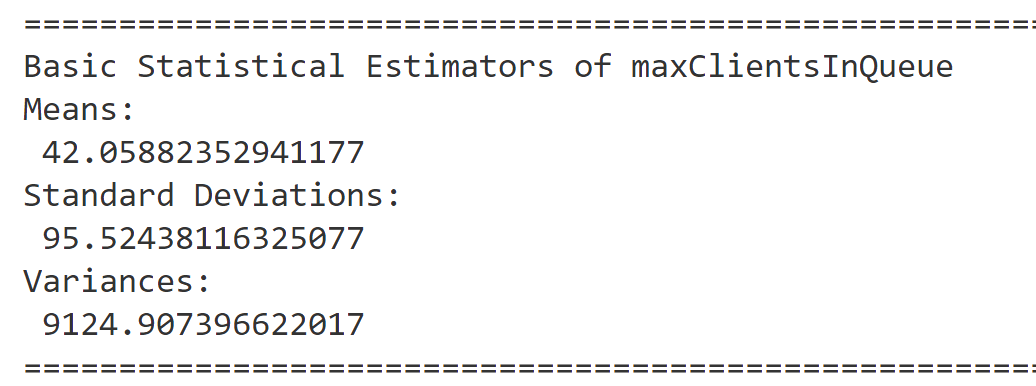
\includegraphics[width=1.2\textwidth]{maximo de clientes en la cola estimadores.png}
\caption{Estimadores de la variable máximo de clientes en la cola}
\end{figure}

\begin{figure}[H]
\centering
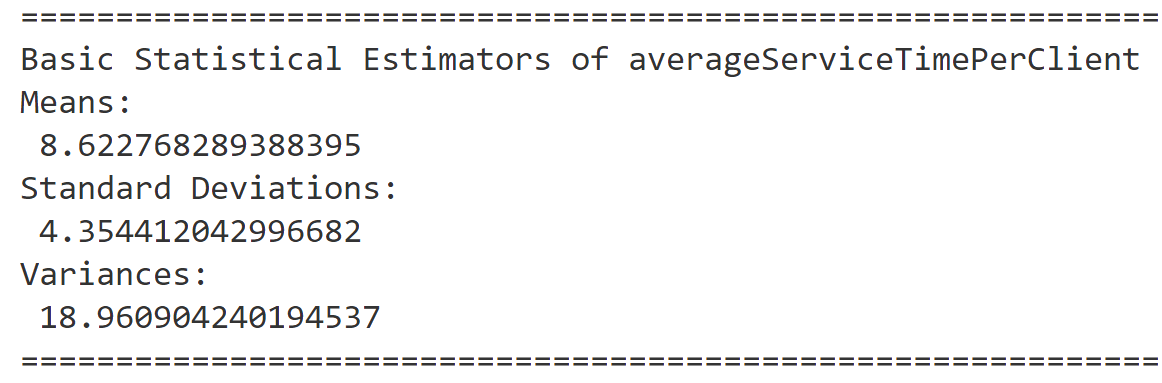
\includegraphics[width=1.2\textwidth]{tiempo de servicio estimadores.png}
\caption{Estimadores de la variable tiempo de servicio}
\end{figure}

\begin{figure}[H]
\centering
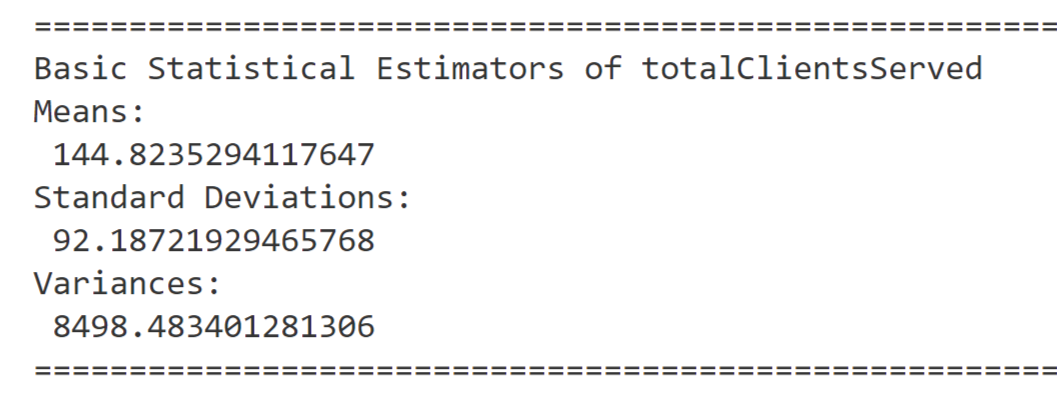
\includegraphics[width=1.2\textwidth]{total de clientes servidos estimadores.png}
\caption{Estimadores de la variable total de clientes atendidos}
\end{figure}

Se calculó la matriz de correlación entre las variables númericas, apoyando la visualización de los resultados con un mapa de calor.

\begin{figure}[H]
\centering
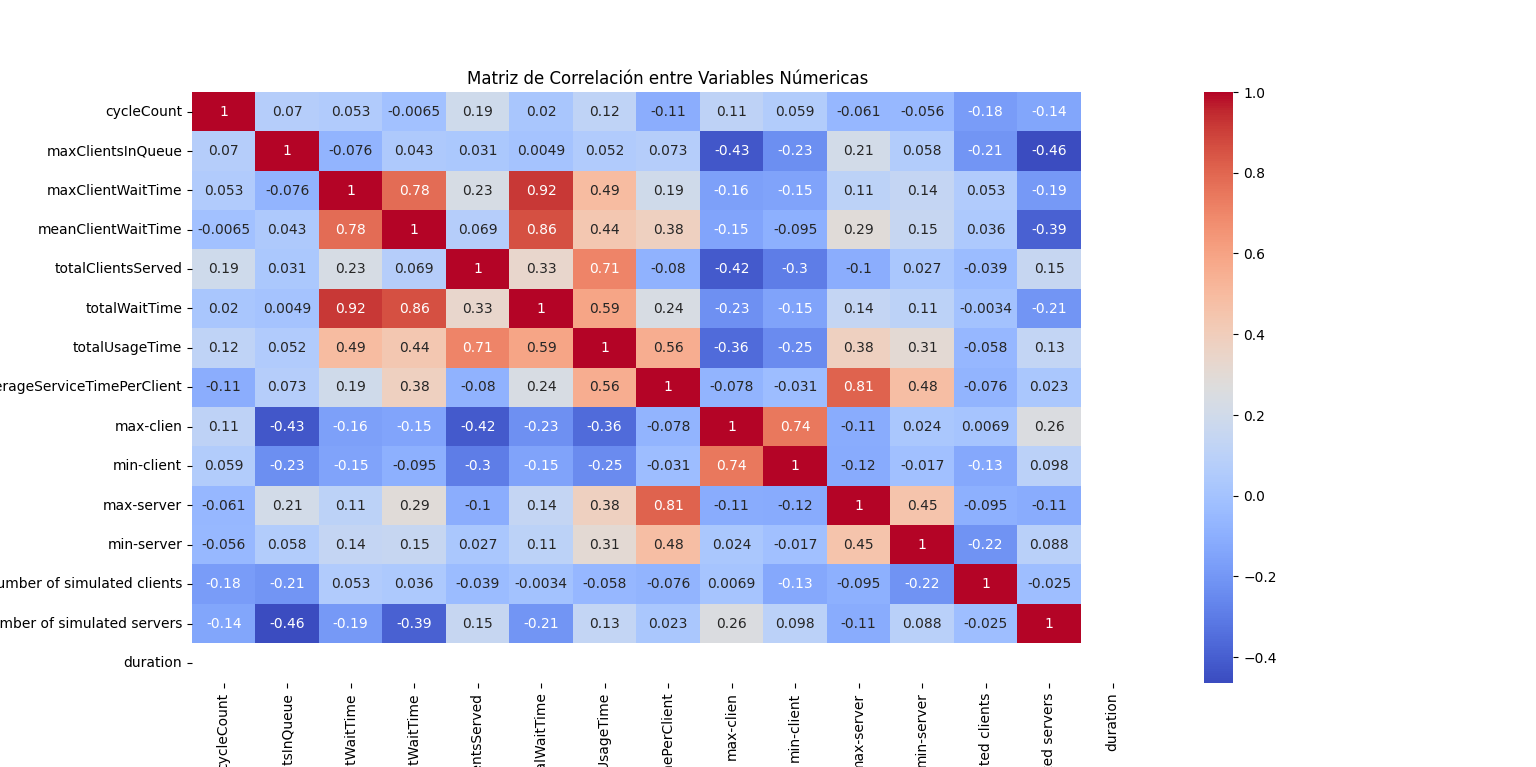
\includegraphics[width=1.2\textwidth]{matriz.png}
\caption{Matriz de correlación}
\end{figure}

En esta se pueden realizar algunas observaciones, como por ejemplo que al aumentar el número de servidores disminuye el tiempo de espera medio y el tiempo de espera máximo. Guiándose igual por la información que brinda y los estimadores extraídos anteriormenete también se puede pensar en disminuir el tiempo de espera aumentando el numero de servidores, lo que a su vez también aumentaría el número de clientes por unida de tiempo. Sin embargo esta y otras observaciones pueden ser evidentes tras un razonamiento lógico, por lo que no haremos énfasis en ellas. 

Se analiza entonces los comportamientos de las variables dependiendo de las distribuciones de clientes y servidores se puede llegar a conclusiones menos evidentes a simple vista. 

\begin{figure}[H]
\centering
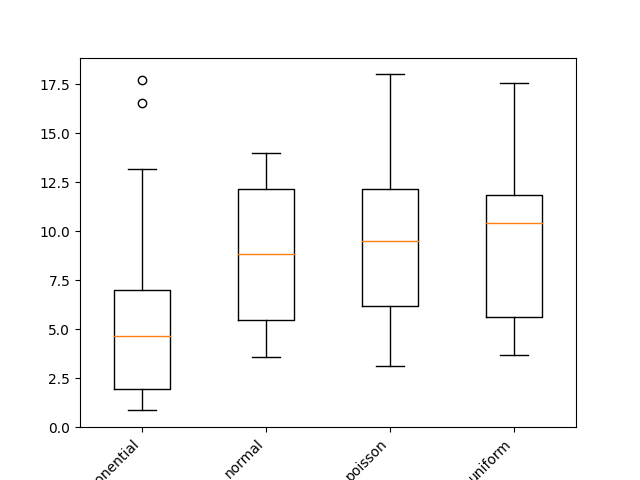
\includegraphics[width=1.2\textwidth]{tiempo x servicio.png}
\caption{Datos agrupados por distribución de servicio de los servidores vs Tiempo de servicio promedio}
\end{figure}

La distribución exponencial es a menudo utilizada para modelar el tiempo de servicio en servidores debido a su propiedad de falta de memoria, lo que significa que el tiempo de servicio no depende del tiempo que ya ha pasado. Esto puede resultar en un tiempo de servicio promedio más bajo si los tiempos de servicio son generalmente cortos. Aquí se puede observar que si los servidores funcionan con ditribución exponencial, el tiempo de servicio promedio de los clientes es más bajo que la media generla de los datos y además mejor que en resto de las distribuciones, siendo esto es un buen resultado.

\begin{figure}[H]
\centering
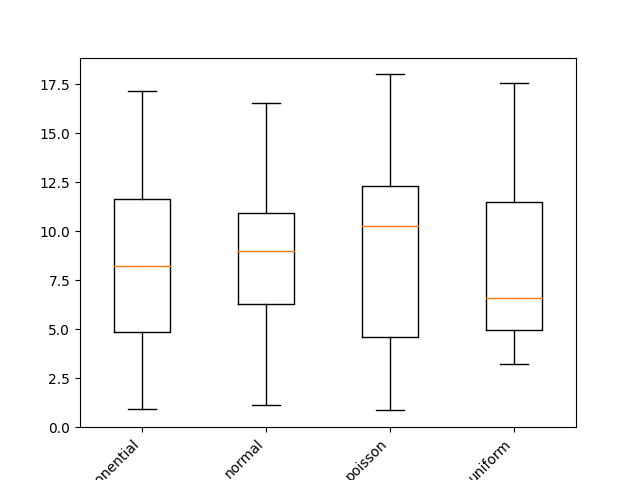
\includegraphics[width=1.2\textwidth]{tiempo x clientes.png}
\caption{Datos agrupados por distribución de llegada de los clientes vs Tiempo de servicio promedio}
\end{figure}

Por otro lado, la distribución de Poisson se utiliza a menudo para modelar la llegada de clientes porque es una buena aproximación para eventos que ocurren de manera aleatoria e independiente a lo largo del tiempo. Sin embargo,  en el caso de las distribuciones por clientes, vemos que la Poisson no posee un valor bajo con respecto a las demás en la media del tiempo de uso del sistema. Si el objetivo es minimizar el tiempo promedio de servicio, puede ser beneficioso utilizar una distribución uniforme (de ser posible) para la llegada de clientes, ya que esto podría resultar en una llegada más predecible y por lo tanto en una menor variabilidad en los tiempos de servicio, lo cual es confirmado por los experimentos ya que se puede observar que es la que menor media posee.

\begin{figure}[H]
\centering
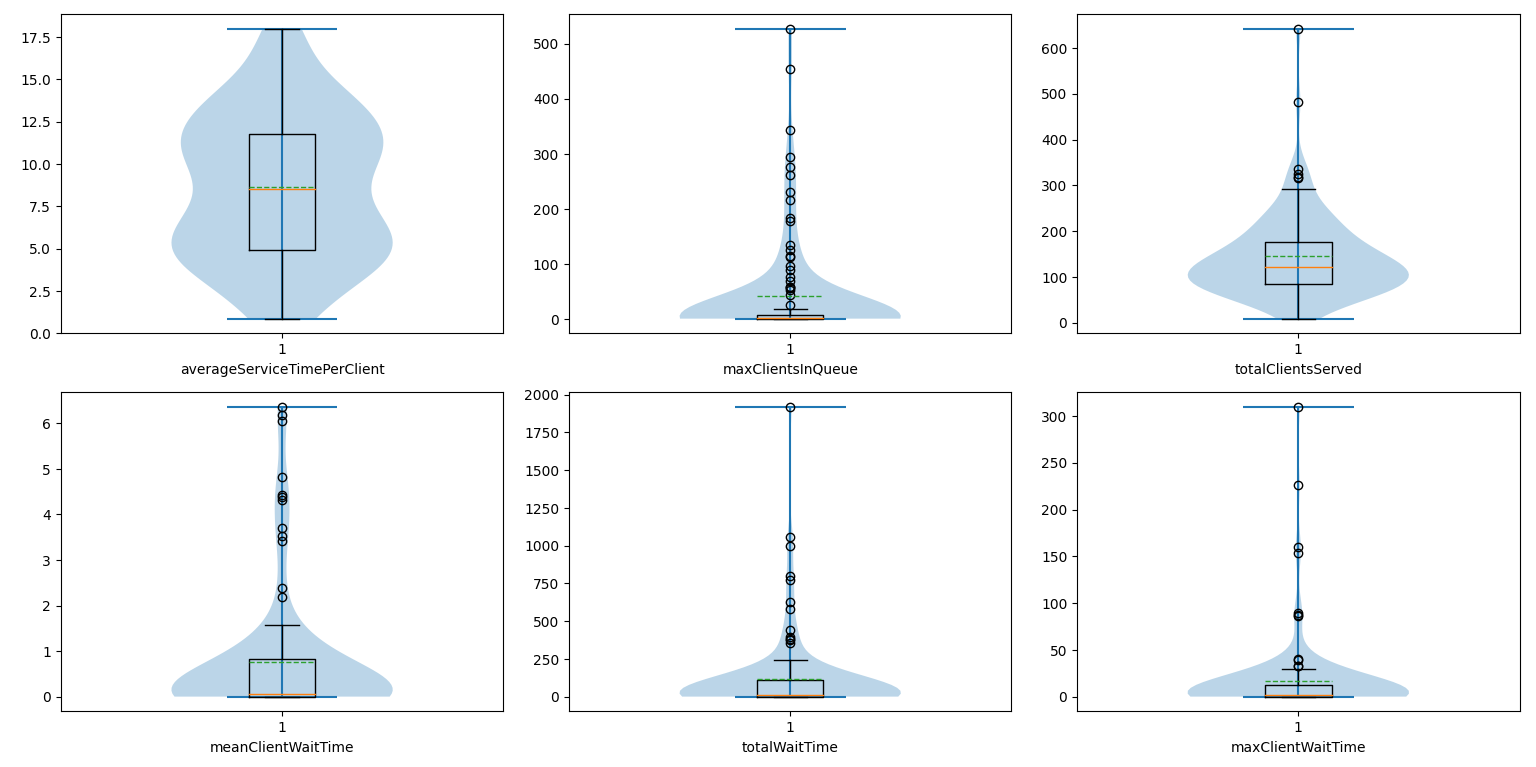
\includegraphics[width=1.2\textwidth]{6.png}
\caption{Visualización de otras variables}
\end{figure}

En el caso de las otras variables vemos que fuera de la cantidad total de clientes atendidos ninguna posee una distribución rápidamente reconocible, en el caso del total de clientes la forma de campana del gráfico de violín parece indicar un comportamiento normal. Si los datos observados en las simulaciones cumplen con las propiedades de una distribución normal, esto podría indicar que el sistema está funcionando de manera eficiente o que los parámetros de la simulación están bien ajustados para modelar el comportamiento real del sistema. La normalidad de los datos puede ser un indicador de que los resultados de las simulaciones son consistentes y que los procesos subyacentes están bien representados por el modelo. Por esto sería interesante realizar un test de normalidad de la variable para así tener un indicador de que otrs resultados del experimento son confiables.

\begin{figure}[H]
\centering
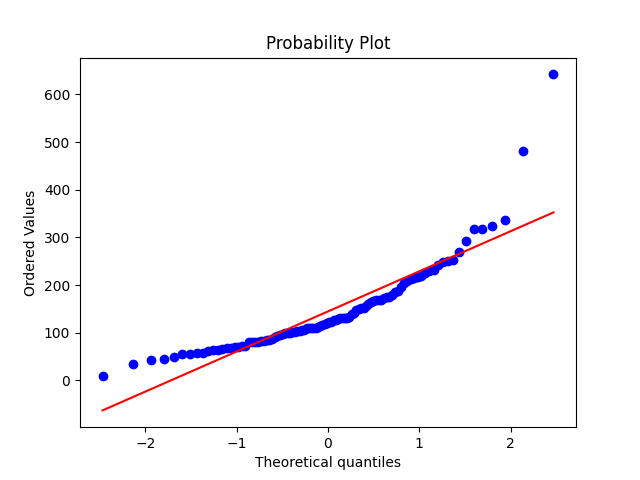
\includegraphics[width=1.2\textwidth]{normal.png}
\caption{Diagrama Q-Q de la variable total de clientes atendidos mostrando posible normalidad}
\end{figure}

\begin{figure}[H]
\centering

\includegraphics[width=1.2\textwidth]{normal-test.png}
\caption{Prueba de hipótesis de normalidad para la variable total de clientes atendidos}
\end{figure}

Como el resultado del test de Durbin no fue el esperado no se recomienda hacer ningún tipo de análisis asumiendo la normalidad de los datos, aunque se propone aumentar el tamaño del conjunto de datos y repetir los tests de normalidad.

\subsection{Necesidad de realizar el análisis estadístico de la simulación}
El análisis estadístico de la simulación de un sistema con servidores en paralelo es esencial por varias razones:
\begin{enumerate}
\item Optimización del rendimiento del sistema: El análisis estadístico puede ayudar a identificar cuellos de botella en el sistema y proporcionar información para optimizar la asignación de clientes a servidores, minimizando así el tiempo de espera y abandono del sistema.
\item Entender el impacto de las distribuciones de llegada y servicio: La distribución (M) para el tiempo entre llegadas y la distribución de servicio en cada servidor (Gi) pueden tener un impacto significativo en el rendimiento del sistema. El análisis estadístico puede ayudar a entender cómo estas distribuciones afectan el rendimiento y proporcionar información para ajustar estas distribuciones si es necesario.
\item Planificación de la capacidad: El análisis estadístico puede proporcionar información sobre la cantidad de servidores necesarios para manejar la carga de trabajo prevista, lo que puede ser útil para la planificación de la capacidad.
\item Mejora de la experiencia del cliente: Minimizar el tiempo de espera y abandono del sistema puede mejorar la experiencia del cliente, lo que puede llevar a una mayor satisfacción del cliente y a una mayor retención de clientes.
\item Toma de decisiones basada en datos: El análisis estadístico proporciona una base sólida para la toma de decisiones, lo que puede llevar a mejores resultados que las decisiones basadas en la intuición o la experiencia.
\end{enumerate}

Cada variable de interés puede dar información que ayude a mejorar el sistema:
\begin{enumerate}
\item cycleCount: Permite rastrear el progreso de la simulación y puede ser útil para identificar patrones o tendencias a lo largo del tiempo.
\item maxClientsInQueue: Indica la capacidad máxima de demanda que el sistema puede manejar sin que los clientes tengan que esperar.
\item maxClientWaitTime: Un tiempo de espera largo puede indicar que el sistema está sobrecargado o que los servidores no están distribuyendo eficientemente su carga de trabajo.
\item meanClientWaitTime: Un tiempo de espera promedio largo puede indicar una eficiencia general baja del sistema.
\item totalClientsServed: Indica cuántos clientes ha podido atender el sistema durante la simulación, lo cual es un indicador directo de su capacidad de procesamiento.
\item totalWaitTime: Un tiempo total de espera largo puede indicar que los clientes están pasando demasiado tiempo en la cola, lo cual puede afectar negativamente su experiencia.
\item totalUsageTime: Ayuda a entender cómo se distribuye el tiempo de trabajo entre los servidores, lo cual puede ser útil para identificar desequilibrios en la carga de trabajo.
\item averageServiceTimePerClient: Un tiempo de servicio promedio largo puede indicar una eficiencia baja en el servicio al cliente.
\item max-client, min-client, max-server, min-server: Estos parámetros definen los límites del sistema y pueden influir en cómo se comporta bajo diferentes condiciones de carga.
\item initial number of simulated clients: Este valor establece el punto de partida para la demanda en el sistema.
\item number of simulated servers: Este valor define la capacidad de procesamiento del sistema.
\item distribution for all service’s time, distribution for i-nth service’s time, distribution for client arrival time: Estas distribuciones pueden ser importantes para modelar la variabilidad en el sistema.
\item duration: Este valor indica el tiempo total durante el cual se ejecutó la simulación, lo cual puede ser útil para comparar diferentes ejecuciones de la simulación.
\end{enumerate}

\subsection{Análisis de parada de la simulación}
La simulación cuenta con diferentes criterios de parada:
\begin{enumerate}
\item Duración de la Simulación: Simplemente se corre la simulación durante un período fijo de tiempo. Esto es útil para comparar el rendimiento del sistema bajo cargas constantes durante un período específico.
\item Número Máximo de Clientes en Cola: Se detiene la simulación si el número máximo de clientes en la cola alcanza un valor crítico, lo que podría indicar una sobrecarga del sistema. Este criterio puede ayudar a identificar el punto de fallo del sistema bajo condiciones de alta demanda.
\item Total de Clientes Atendidos: Se detiene la simulación después de que un cierto número de clientes ha sido atendido. Esto puede ser particularmente relevante para evaluar la capacidad total del sistema para manejar una carga de trabajo
\end{enumerate}


\section{Modelo matemático}

El modelo matemático que mejor se ajusta a este problema es el Modelo de Colas. 
\begin{figure}[H]
\centering
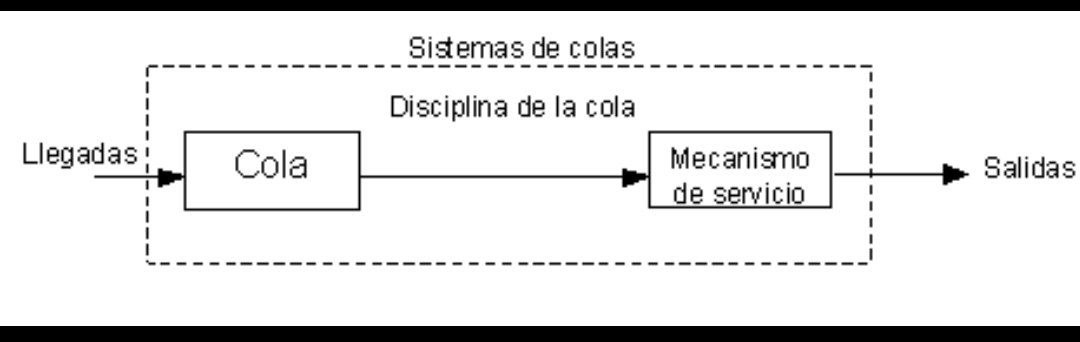
\includegraphics[width=1.2\textwidth]{modelo.jpg}
\caption{Modelo base de Teoría de colas}
\end{figure}

\subsection{Descripción del modelo de simulación}

Los clientes que requieren un servicio se generan en el tiempo en una fuente de entrada.
Luego, entran al sistema y se unen a una cola. En determinado momento se selecciona
un miembro de la cola para proporcionarle el servicio mediante alguna regla conocida como
disciplina de la cola. Se lleva a cabo el servicio que el cliente requiere mediante un mecanismo
de servicio, y después el cliente sale del sistema de colas.

Llamamos tamaño de la fuente de entrada al número total de clientes que pueden
requerir servicio en un determinado momento. Podemos suponer que el tamaño es finito o
infinito. Se especifica el patrón estadístico mediante el cual se generan los clientes a
través del tiempo.

La cola es el lugar donde los clientes esperan antes de recibir el servicio. Esta posee dos
caracteríısticas principales, en primer lugar la capacidad de la cola, es decir, el número máximo
de clientes que puede llegar a soportar. Esta capacidad puede ser finita o infinita.

La disciplina de la cola se refiere al orden en el que sus miembros se seleccionan para
recibir el servicio.Los modelos más importantes son los siguientes:
FIFO (First-In-First-Out): se le da servicio al primero que ha llegado, de forma que la
cola está ordenada según el orden de llegada de los usuarios.
LIFO (Last-In-First-Out): se le da servicio al último que ha llegado, de forma que la
cola está ordenada en orden inverso al de llegada de los usuarios.
SIRO (Service-In-Random-Order): se sortea aleatoriamente cuál de los usuarios en
espera accederá al servicio.
No obstantes, otro procedimiento para establecer la disciplina de la cola puede ser el
de establecer determinadas prioridades a los diferentes usuarios según algunas de sus características.
En sistemas finitos, en los que el número de usuarios en espera es limitado, es necesario
establecer además qué sucede con aquellos usuarios que acceden al sistema cuando la cola
de espera está completa. Por último, en los sistemas en que los usuarios son humanos, hay
que tener en cuenta otros factores propios del comportamiento humano como el hecho de
que hay individuos que no respetan el orden establecido en la cola o bien que hay usuarios
que, a la vista de la cola, renuncian a acceder al sistema.


El mecanismo de servicio consiste en una o más estaciones de servicio, cada una de ellas
con uno o más servidores o canales de servicio paralelos, llamados servidores. Si el tiempo que tardan
los usuarios en salir del sistema es mayor que el intervalo entre llegadas, la cola aumentará
indefinidamente y el sistema puede llegar a colapsarse. 

Los modelos más elementales suponen una estación, ya sea con un servidor o con un
número finito de servidores. Se llama tiempo de servicio al
tiempo que transcurre desde el inicio del servicio para un cliente hasta su terminación en
una estación . Se especifica la distribución
de probabilidad de los tiempos de servicio de cada servidor (y tal vez de los distintos tipos
de clientes), aunque es común suponer la misma distribución para todos los servidores. 


\subsection{Supuestos y restricciones}

En este caso se simula un  modelo de colas basados en el proceso de nacimiento y muerte (potencialmente infinito si se elimina la restricción de máximo número de clientes en cola) con uno o más servidores. En estos modelos se supone que todos los tiempos entre llegadas son independientes e
idénticamente distribuidos de acuerdo con una distribución (usualmente en la práctica el proceso
de entrada es de Poisson, aunque se decidió experimentar con otras distribuciones), que todos los tiempos de servicio son idependientes e idénticamente
distribuidos de acuerdo con otra distribución (nuevamente aunque en la vida real la más usada es la  exponencial, se experimentó además con otras ) y que el número de servidores es cualquier entero positivo.  El modelo de disciplina implementado es FIFO (First-In-First-Out): se le da servicio al primero que ha llegado, de forma que la
cola está ordenada según el orden de llegada de los usuarios.

Algunos de los supuestos del proyecto fueron:
\begin{enumerate}
\item Independencia de Llegadas: Se asume que los tiempos de llegada de los clientes son independientes entre sí.
\item Capacidad de los Servicios: Se asume que cada servidor puede atender a un número ilimitado de clientes, lo que significa que la capacidad de los servidores es infinita, aunque siempre de uno en vez.
\item Tiempo de Espera en Cola: Se asume que el tiempo de espera en la cola es el tiempo que un cliente pasa en la cola antes de ser atendido.
\end{enumerate}

\section{Bibliografía}
Modelos de teorías de colasS. Gabriel Esteban Velázquez. Facultad de  Matemáticas. Departamento de estadística e investigación operativa. Universidad de Sevilla
 \href{https://idus.us.es/bitstream/handle/11441/77595/Esteban%20Vel%C3%A1zquez%20Gabriel%20TFG.pdf?sequence=1&isAllowed=y}{link al paper}

Intorducción a la teoría de colas y su simulación.Gerardo Fabian Peraza Siqueiros.División de Ciencias Exactas y Naturales.Departamento de Matemáticas. Universidad de Sonora.
 \href{https://lic.mat.uson.mx/tesis/044_Gerardo_FabianPS.pdf}{link al paper}





\end{document}
